\def\RIC{\RICTXT}

% #########################################
% #########################################
\def\MXCOL{black}
\def\FXCOL{Orchid3}
\def\MNCOL{SeaGreen4}
\def\FNCOL{SeaGreen4}
\def\NCOL{SeaGreen4}
\def\XCOL{Tomato}
\def\WCOL{Tomato}
\def\YCOL{DodgerBlue4}
\def\TEXTCOL{gray}
\def\AXISCOL{white}
% ###########################################################
% ###########################################################
% \ifFIGS
% \begin{figure}[t]
%   \tikzexternalenable
%   \tikzsetnextfilename{occur}
%   \vspace{-0pt}
%   \centering 

%   \iftikzX
%   \begin{tikzpicture}[font=\bf\sffamily\fontsize{8}{10}\selectfont]
  \def\TEXTCOL{gray}
  \tikzset{
    hatch distance/.store in=\hatchdistance,
    hatch distance=20pt,
    hatch thickness/.store in=\hatchthickness,
    hatch thickness=2pt
  }

  % \makeatletter
  % \pgfdeclarepatternformonly[\hatchdistance,\hatchthickness]{flexible hatch}
  % {\pgfqpoint{0pt}{0pt}}
  % {\pgfqpoint{\hatchdistance}{\hatchdistance}}
  % {\pgfpoint{\hatchdistance-1pt}{\hatchdistance-1pt}}%
  % {
  %   \pgfsetcolor{\tikz@pattern@color}
  %   \pgfsetlinewidth{\hatchthickness}
  %   \pgfpathmoveto{\pgfqpoint{0pt}{0pt}}
  %   \pgfpathlineto{\pgfqpoint{\hatchdistance}{\hatchdistance}}
  %   \pgfusepath{stroke}
  % }
  % \makeatother
  % \pgfdeclarepatternformonly{north east lines wide}%
  % {\pgfqpoint{-1pt}{-1pt}}%
  % {\pgfqpoint{10pt}{10pt}}%
  % {\pgfqpoint{9pt}{9pt}}%
  % {
  %   \pgfsetlinewidth{0.4pt}
  %   \pgfpathmoveto{\pgfqpoint{0pt}{0pt}}
  %   \pgfpathlineto{\pgfqpoint{9.1pt}{9.1pt}}
  %   \pgfusepath{stroke}
  % }

  \def\HGTPP{1.4in}
  \def\HGTX{1.35in}
  \def\HGTXx{1.5in}
  \def\HGTWW{1.35in}
  \def\WDTX{3in}
  \def\HGT{1.35in}
  \def\WDTC{3.35in}
  \def\WDT{3in}
  \def\WDTH{1.5in}
  \def\HGTH{3.650in}
  \def\CHLPREV{../../data_latest/figfiles/prev_combined}
  \def\CHLPREVN{../../data_latest/figfiles/prev_combined_norm}
  \def\DATAA{../../data/figfiles/diffinit.csv}
  \def\BWDT{5.5pt}
  \def\LENDATA{../../data/figfiles/LEN.csv}
  \def\CDCDATA{../../data/figfiles/cdc_prevalence.csv}
  \def\CODEDATA{../../data/figfiles/propcode.csv}

  \node[] (A0) at (0,0.0) {};
  \node [anchor=north] (A) at (A0.south) {\includegraphics[width=\WDTC]{\CHLPREV}};
  \node [anchor=north] (B) at ([yshift=-0.15in]A.south) {\includegraphics[width=\WDTC]{\CHLPREVN}};

  \node[anchor=north east] (D) at ([xshift=-0.5in,yshift=-.25in]A.north west) {
   \def\BANDCOLB{DarkOrange!80}
  \def\BANDCOLB{Yellow2}
  \def\BANDCOL{lightgray}
  \def\PLOTCOL{black}
  \def\AXISCOL{black!20}
  \def\HGT{1.1in}
  \def\WDT{1.15in}
  \def\OPC{1}
  \def\BWIDTH{9pt}
        \begin{tikzpicture}[anchor=west,text=\TEXTCOL]
 % \clip (0in,-0.4in) rectangle (2.65in,-3.65in);
\def\datafileP{../../data/figfiles/pf_yr.csv}
\def\datafileU{../../data/figfiles/ub_yr.csv}
\def\datafileL{../../data/figfiles/lb_yr.csv}
 \begin{axis}[legend cell align=left,name=XA, font=\bf\sffamily\fontsize{8}{8}\selectfont, 
        title={Infections},
    title style={},
    legend style={at={(1,1)}, xshift=0in, yshift=0in, draw=white, fill=white, fill opacity=1, 
      text opacity=1,},
    axis line style={\AXISCOL, opacity=0,ultra  thick, rounded corners=0pt},
    axis on top=false, 
    grid style={dashed, gray!40},
    enlargelimits=false, 
    width=\WDT, 
    height=\HGT,     % size of the image
     ymin=-30,
     ymax=60,
     xmax=6,
     % ymax=1.275,
     % ymin=.99,
    scale only axis=true,
     grid,
    xlabel={age [yr]},
    yticklabel style={xshift=-.015in},
    ylabel style={yshift=-.1in},
    xlabel style={yshift=.0in},
    %ylabel={\% increase in incidence in treatment vs control},
    scaled x ticks = false,
     x tick label style={yshift=-.05in,/pgf/number format/fixed,
    /pgf/number format/1000 sep = %\thinspace % Optional if you want to replace comma as the 1000 separator 
     },
     major tick length=0pt,
    ];
    % 
    \addplot[ smooth, ultra thick, \MXCOL,mark=*, opacity=.85,
    mark options={%
      scale=1.5,draw=black,  thick, fill=white,  opacity=1,
    },]table[x expr=(\coordindex+1),y=INFM,col sep=comma]
    {\datafileP};
    \addlegendentry{Male};
    \addplot[ smooth, ultra thick, \FXCOL,mark=*, opacity=.85,
    mark options={%
      scale=1.5,draw=\FXCOL,  thick, fill=white,  opacity=1,
    },]table[x expr=(\coordindex+1),y=INFF,col sep=comma]
    {\datafileP};
    \addlegendentry{Female};
     \addplot[smooth, draw=none,,name path=Ax]table[x expr=(\coordindex+1),y=INFM,col sep=comma]
    {\datafileU};
    \addplot[smooth,  draw=none,,name path=Bx]table[x expr=(\coordindex+1),y=INFM,col sep=comma]
    {\datafileL};
    \addplot[\BANDCOL,opacity=.5] fill between[of=Ax and Bx];
     \addplot[smooth, draw=none,,name path=Ay]table[x expr=(\coordindex+1),y=INFF,col sep=comma]
    {\datafileU};
    \addplot[smooth,  draw=none,,name path=By]table[x expr=(\coordindex+1),y=INFF,col sep=comma]
    {\datafileL};
    \addplot[\BANDCOL,opacity=.5] fill between[of=Ay and By];
  \end{axis}
  \begin{axis}[legend cell align=left,name=XB, font=\bf\sffamily\fontsize{8}{8}\selectfont,
    title={Immunologic},
    title style={},
    at=(XA.north east),anchor=north west,xshift=0.5in,
    legend style={at={(1,1)}, xshift=0in, yshift=0in, draw=white, fill=white, fill opacity=1, 
      text opacity=1,},
    axis line style={\AXISCOL, opacity=0,ultra  thick, rounded corners=0pt},
    axis on top=false, 
    grid style={dashed, gray!40},
    enlargelimits=false, 
    width=\WDT, 
    height=\HGT,     % size of the image
     ymin=-30,
     ymax=60,
     xmax=6,
     % ymax=1.275,
     % ymin=.99,
    scale only axis=true,
     grid,
    xlabel={age [yr]},
    yticklabel style={xshift=-.015in},
    ylabel style={yshift=-.1in,xshift=-.7in},
    xlabel style={yshift=.0in},
    %ylabel={\% increase in incidence in treatment vs control},
    scaled x ticks = false,
     x tick label style={yshift=-.05in,/pgf/number format/fixed,
    /pgf/number format/1000 sep = %\thinspace % Optional if you want to replace comma as the 1000 separator 
     },
     major tick length=0pt,
    ];
    % 
    \addplot[ smooth, ultra thick, \MXCOL,mark=*, opacity=.85,
    mark options={%
      scale=1.5,draw=black,  thick, fill=white,  opacity=1,
    },]table[x expr=(\coordindex+1),y=IMMM,col sep=comma]
    {\datafileP};
    \addlegendentry{Male};
    \addplot[ smooth, ultra thick, \FXCOL,mark=*, opacity=.85,
    mark options={%
      scale=1.5,draw=\FXCOL,  thick, fill=white,  opacity=1,
    },]table[x expr=(\coordindex+1),y=IMMF,col sep=comma]
    {\datafileP};
    \addlegendentry{Female};
     \addplot[smooth, draw=none,,name path=A]table[x expr=(\coordindex+1),y expr=(\thisrow{IMMM} *1.3),col sep=comma]
    {\datafileU};
    \addplot[smooth,  draw=none,,name path=B]table[x expr=(\coordindex+1),y expr=(\thisrow{IMMM} *.9,col sep=comma]
    {\datafileL};
    \addplot[\BANDCOL,opacity=.5] fill between[of=A and B];
     \addplot[smooth, draw=none,,name path=A]table[x expr=(\coordindex+1),y expr=(\thisrow{IMMF}+(25/(\coordindex+1))),col sep=comma]
    {\datafileU};
    \addplot[smooth,  draw=none,,name path=B]table[x expr=(\coordindex+1),y expr=(\thisrow{IMMF} *.5),col sep=comma]
    {\datafileL};
    \addplot[\BANDCOL,opacity=.5] fill between[of=A and B];
  \end{axis}
      \end{tikzpicture}
  %   \begin{tikzpicture}[]

  %     \begin{groupplot}[group style={horizontal sep=.1in,group name=A,group size= 2 by 1},title style={text=\TEXTCOL},
  %       legend style={anchor=east,at={(0,1.05)},
  %         inner sep=3pt,draw=none,fill=white,fill opacity=.85,
  %         align=right,text opacity=1,
  %         font=\bf\sffamily\fontsize{8}{9}\selectfont},
  %       axis line style={lightgray, opacity=0, thin},%
  %       % grid,
  %       % xshift=.5in,
  %       % anchor=north west,
  %       height=\HGTH,
  %       width=\WDTH,
  %       xbar, 
  %       ytick=data,% crucial line for the xticklabels directive 
  %       % ymin=0,
  %       yticklabel style={font=\bf\sffamily\fontsize{7}{7}\selectfont,align=right, yshift=0in,xshift=0in,text=\TEXTCOL},
  %       major tick length=0pt,
  %       xticklabel style={font=\bf\sffamily\fontsize{8}{7}\selectfont,text=\TEXTCOL},
  %       grid,
  %       grid style={lightgray, opacity=.5},
  %       axis on top=false,xlabel={control $\leftarrow \Delta$ \% prevalence $\rightarrow$ positive},xlabel style={yshift=0.05in,xshift=-.15in,text=\TEXTCOL},
  %       enlarge y limits=0.05,enlarge x limits=0
  %       ] 
  %       \nextgroupplot[%title={50 weeks},      %  xmin=-5,xmax=5,
  %       bar width=\BWDT, yticklabels from table={\DATAA}{disease},]
  %       \addplot[opacity=1,fill=\MXCOL, draw=none,area legend] table [ 
  %       y expr=\coordindex,
  %       x=M
  %       ] {\DATAA};   
  %       \addlegendentry{Male}
  %       \addplot[opacity=1,fill=\FXCOL, draw=none,area legend] table [ 
  %       y expr=\coordindex,
  %       x=F
  %       ] {\DATAA};   
  %       \addlegendentry{Female}

  %       % \nextgroupplot[title={150 weeks},        xmin=-5,xmax=5,
  %       % yticklabel=\empty, bar width=\BWDT, yticklabels from table={\DATAC}{disease}, yticklabel=\empty,xlabel={}]
  %       % \addplot[opacity=1,fill=\MXCOL,draw=none, area legend] table [ 
  %       % y expr=\coordindex,
  %       % x=M
  %       % ] {\DATAC};   
  %       % % \addlegendentry{Male}
  %       % \addplot[opacity=1,fill=\FXCOL,draw=none, area legend] table [ 
  %       % y expr=\coordindex,
  %       % x=F
  %       % ] {\DATAC};   
  %       % % \addlegendentry{Female}

  %     \end{groupplot} 

  %   \end{tikzpicture}
   };

  
 %  \node[anchor=north west] (C) at ([yshift=-0.2in,xshift=0.5in]D.south west) {
%     \begin{tikzpicture}[]
%       \begin{axis}[legend cell align=left,legend style={anchor=east,at={(0.65,0.85)},inner sep=3pt,draw=none,fill=white,fill opacity=.85,align=right,text opacity=1,font=\bf\sffamily\fontsize{8}{9}\selectfont},
%         axis line style={lightgray, opacity=0.8, very thick},%
%         enlargelimits=true,
%         height=1.4in,
%         width=3.5in,
%         % enlarge x limits=0.03,
%         %ybar,bar width=18pt,    
%         major tick length=0pt,
%         xlabel={year of survey},axis x line=bottom,
%         axis y line=left,
%         ymin=5,
%         %xmax=500,
%         xticklabel style={font=\bf\sffamily\fontsize{7}{7}\selectfont,text=\TEXTCOL},
%         grid,
%     grid style={dashed,gray!40},
%         %grid style={lightgray, opacity=.5},
%         %grid style={lightgray, dashed, opacity=.6},
%         axis on top=false, 
%         ylabel={}, x tick label style={yshift=-0.02in,text=\TEXTCOL},
%         xlabel style={yshift=0.05in,text=\TEXTCOL},
% ylabel style={yshift=-.05in,text=\TEXTCOL},y tick label style={,text=\TEXTCOL,xshift=.0in,/pgf/number format/fixed,/pgf/number format/precision=0,/pgf/number format/fixed zerofill,
%           /pgf/number format/1000 sep = %\thinspace % Optional if you want to replace comma as the 1000 separator 
%         },x tick label style={/pgf/number format/fixed,/pgf/number format/precision=0,/pgf/number format/fixed zerofill,          /pgf/number format/1000 sep = %\thinspace % Optional if you want to replace comma as the 1000 separator 
%         },enlarge x limits=0.1]
%         \addplot[opacity=.8, draw=\MXCOL,ultra thick,%fill=\WCOL,
%         mark=*,
%         mark options={      scale=1.95,draw=\MXCOL,  thick, fill=white,  opacity=1,
% }
%         ] table [%
%         x=syear,
%         y=prev1000
%         ] {\CDCDATA};   
% \draw [ ultra thick,draw=Tomato] (axis cs:2013,\pgfkeysvalueof{/pgfplots/ymin}) -- (axis cs:2013,\pgfkeysvalueof{/pgfplots/ymax})  node[midway,left,fill=white,pos=.3] {DSM V};
%        % \addlegendentry{prevalence/1000}
%      \end{axis}
%     \end{tikzpicture}
%   };

  \node[anchor=north west] (E) at ([xshift=.45in,yshift=-.5in]D.south west) {
    \begin{tikzpicture}[]
      \begin{axis}[legend cell align=left,anchor=center,legend style={anchor=east,at={(0.75,0.8)},inner sep=3pt,draw=none,fill=white,fill opacity=.85,align=right,text opacity=1,font=\bf\sffamily\fontsize{8}{9}\selectfont},axis line style={lightgray, opacity=0, thin},%
        enlargelimits=true,
        height=2.4in,
        width=3.25in,
        % enlarge x limits=0.03,
        ybar,bar width=2.5pt,    
        major tick length=0pt,
        xlabel={ASD diagnosis age [weeks]},
        xmin=100,
        xmax=500,
        xticklabel style={font=\bf\sffamily\fontsize{7}{7}\selectfont,text=\TEXTCOL},
        % grid,
        grid style={lightgray, opacity=.7},
        axis on top=false, 
        ylabel={probability}, x tick label style={yshift=0.0in,text=\TEXTCOL},
        xlabel style={yshift=0in,text=\TEXTCOL},ylabel style={xshift=-0.45in,text=\TEXTCOL},y tick label style={,text=\TEXTCOL,xshift=.0in,/pgf/number format/fixed,/pgf/number format/precision=2,/pgf/number format/fixed zerofill,
          /pgf/number format/1000 sep = %\thinspace % Optional if you want to replace comma as the 1000 separator 
        },]
        \addplot[opacity=1,fill=\MXCOL, draw=none,area legend] table [col sep=comma,
        x=LEN,
        y=M
        ] {\LENDATA};   
        \addlegendentry{Male}
        \addplot[opacity=1,fill=\FXCOL,draw=none, area legend] table [col sep=comma,
        x=LEN,
        y=F
        ] {\LENDATA};   
         \addlegendentry{Female}
     \end{axis}
    \end{tikzpicture}
  };



%     \node[anchor=north west] (F) at ($(E.north west)!(C.north west)!(E.north east)$) {
%     \begin{tikzpicture}[]
%       \begin{axis}[legend cell align=left,legend style={anchor=east,at={(0.4,1.05)},
%           inner sep=3pt,draw=none,fill=white,fill opacity=.85,
%           align=right,text opacity=1,
%           font=\bf\sffamily\fontsize{8}{9}\selectfont},,axis line style={lightgray, opacity=0, thin},%
%         height=\HGTPP, width=\WDT,
%         ybar,bar width=3pt,    
%         major tick length=0.0pt,
%         xlabel={fraction of weeks with heathcare event},
%         %xmin=100,
%         enlargelimits=true,
%         xmax=0.45,
%         xticklabel style={font=\bf\sffamily\fontsize{7}{7}\selectfont,text=\TEXTCOL},
%         % grid,
%         grid style={lightgray, opacity=.7},
%         axis on top=false, 
%         ylabel={probability}, x tick label style={yshift=0.05in,text=\TEXTCOL},
%         xlabel style={yshift=0.0in,text=\TEXTCOL},ylabel style={yshift=-0in,xshift=-.45in,text=\TEXTCOL},x tick label style={,text=\TEXTCOL,xshift=.1in,yshift=-.05in,/pgf/number format/fixed,/pgf/number format/precision=2,/pgf/number format/fixed zerofill,
%           /pgf/number format/1000 sep = %\thinspace
%         },y tick label style={text=\TEXTCOL,/pgf/number format/fixed,/pgf/number format/precision=2,/pgf/number format/fixed zerofill,
%           /pgf/number format/1000 sep = %\thinspace 
%         },scaled ticks=false, enlarge y limits=0.07,enlarge x limits=0,
%         ]
%         \addplot[opacity=.7,fill=\MNCOL, draw=none,area legend] table [col sep=comma,
%         y=M,
%         x=proportionNz
%         ] {\CODEDATA};   
% %        \addlegendentry{Male}
%         % \addplot[opacity=1,fill=\FXCOL,draw=none, area legend] table [col sep=comma,
%         % y=proportionNz,
%         % x=F
%         % ] {\CODEDATA};   
%         %  \addlegendentry{Female}
%      \end{axis}
%     \end{tikzpicture}
%   };


  \node[anchor=south west,align=left] (LA) at ([xshift=0.25in,yshift=-0.1in]A.north west) {{\LARGE C.} Autism Insurance Claims 2003-2013\\(source: Truven Marketscan)};
  \node[anchor=south west,align=left] (LB) at ([yshift=-0.1in]$(LA.north west)!(B.north west)!(LA.south west)$) {{\LARGE D.} Autism Prevalence in US (Population Normalized) };
   \node[anchor=north west,align=left] (LD) at ([xshift=.5in]$(LA.north west)!(D.north west)!(LA.north east)$) {{\LARGE A.} Population-level Prevalence Differences\\between Positive vs Control Populations};
   % \node[anchor=north west,align=left] (LF) at ([yshift=0.25in]$(LD.north west)!(F.north west)!(LD.south west)$) {{\LARGE E.} Diagnostic Code Fraction Available per Patient};
   \node[anchor=north west,align=left] (LC) at ([yshift=0in]$(LB.north west)!(LD.north west)!(LB.north east)$) {{\LARGE B.}
%Autism Prevalence per 1000 (source: CDC)};
     %\node[anchor=south west,align=left] (LE) at ([yshift=-.1in]$(LC.north west)!(E.north west)!(LC.south west)$)
     %{{\LARGE E.}
       ASD Clinical Diagnosis Age Across Genders };

\end{tikzpicture}
   
%   \else
%   \includegraphics[width=0.9\textwidth]{Figures/External/occur}
%   \fi
   
%   \captionN{ASD Occurrence Patterns. 
%     Panel A illustrates the differential representation of different disease categories in the \treatment and control cohorts, and panel B shows the distribution of the age of  diagnosis for males and females in the Truven dataset. Panel C illustrates the spatial distribution of ASD insurance claims, and panel D shows the same data after population normalization, illustrating the relatively small demographic skew to ASD prevalence within the general population with access to medical insurance, which is consistent with the suggestion that prevalence variation might be linked to regional and socioeconomic disparities in access to services~\cite{jarquin2011racial}.
%   }\label{EXT-fig0}
% \end{figure}
% \else
% \refstepcounter{figure}\label{EXT-fig0}
% \fi
% ###########################################################
% ###########################################################
% ##########################################
\begin{table*}[!ht]
  % \mnp{\textwidth}{
  \captionN{Patient Numbers, Inclusion-exclusion Criteria and Features Used In Analysis}
    \begin{subtable}{\textwidth}
  \begin{center}
    \captionN{Patient Counts In De-identified Data \& The Fraction of Datasets Excluded By Our Exclusion Criteria$^\star$}\label{tab2}
    \sffamily\small
    \begin{tabular}{L{1.5in}L{.695in}L{.695in}C{.695in}L{.695in}L{.695in}}
      &\multicolumn{2}{c@{\quad}}{Truven}    
      &&                                           
         \multicolumn{2}{c}{UCM} \\\cline{2-3}\cline{5-6}          
      Distinct Patients &\multicolumn{2}{c@{\quad}}{115,805,687}    
      &&                                           
         \multicolumn{2}{c}{69,484} \\\cline{2-3}\cline{5-6}          
      &Male& Female    && Male  &Female      \\
      \hline
      ASD Diagnosis Count$^\dag$ & 12,146 & 3,018& &307& 70 \\\hline
      Control Count$^\dag$ & 2,301,952 & 2,186,468 & & 20,249& 17,386\\\hline
      AUC at 125 weeks & 82.3\% & 82.5\% & &83.1\%& 81.37\%\\\hline
      AUC at 150 weeks & 84.79\% & 85.26\% & &82.15\%& 83.39\%\\\hline
      &&     &  &   &      \\
      \multicolumn{5}{c}{Excluded Fraction of the Data sets}      &      \\
      &&     &  &   &      \\
      \hline
      Positive Category & 0.0002 & 0.0& &0.0160& 0.0 \\\hline
      Control Category & 0.0045 &0.0045 & &0.0413&  0.0476\\\hline

      &&     &  &   &      \\
      \multicolumn{6}{c}{Average Number of Diagnostic Codes In Excluded Patients (corresponding number in included patients)}           \\
      &&     &  &   &      \\
      \hline
      Positive Category & 4.33 (35.93) & 0.0 (36.07)& &2.6 (9.75)& 0.0 (10.18) \\\hline
      Control Category & 1.57 (17.06) & 1.48 (15.96)  & & 2.32 (6.8)& 2.07 (6.79) \\\hline

    \end{tabular}


  \end{center}
    \vskip .5em
  \small
  $^\dag$ Cohort sizes are smaller than the total number of distinct patients due to the following exclusion criteria: 1) At least one code within our complete set of tracked diagnostic codes is present in the patient record, 2) Time-lag between first and last available record for a patient is at least 15 weeks.

  $^\star$ Dataset sizes are after the exclusion criteria are applied

\end{subtable}
\vskip 1em
% %}

% \end{table*}
% % ###########################################################
% % ###########################################################% ###########################################################
% \begin{table*}[t]
%\mnp{\textwidth}{
  \begin{subtable}{\textwidth}
%\begin{center}  
  \captionN{Engineered Features (Total Count: 165)}\label{EXT-tab1}
  \vskip .5em

  \begin{tabular}{L{2.25in}|L{3in}|C{1in}} \hline
    \textbf{Feature Type$^\ddag$}               & \textbf{Description}   & \textbf{No. of Features}   \\\hline
    {[}Disease Category{]}$_{ \ \Delta}$               & Likelihood Defect (See Methods section) & 17   \\\hline
    {[}Disease Category{]}$_{ \ 0}$               & Likelihood of control model (See Methods section) & 17  \\\hline
    {[}Disease Category{]}$_{\textrm{ proportion}}$   & Occurrences in the encoded sequence / length of the sequence         & 17\\\hline
    {[}Disease Category{]}$_{\textrm{ streak}}$      & Maximum Length of adjacent occurrences  of {[}Disease Category{]}    & 51      \\\hline
    {[}Disease Category{]}$_\textrm{ prevalence}$   &  Maximum, mean  and variance of Occurrences in the encoded sequence / Total Number of diagnostic codes in the mapped sequence   & 51      \\\hline
    Feature Mean, Feature Variance, Feature Maximum for difference of control and case models                 & Mean, Variance, Maximum of the {[}Disease Category{]}$_{ \ \Delta}$ values   & 3     \\\hline
    Feature Mean, Feature Variance, Feature Maximum for control models               & Mean, Variance, Maximum of the {[}Disease Category{]}$_{\ 0}$ values   & 3     \\\hline
    Streak      & Maximum, mean  and variance of the length of adjacent occurrences  of {[}Disease Category{]}    & 3      \\\hline
    Intermission& Maximum, mean  and variance of the length of adjacent empty weeks     & 3    \\\hline
  \end{tabular}
  %\end{center}
  \vskip .5em
  \small
  $^\ddag$ Disease categories are described in Table~\ref{SI-tab0}
 \end{subtable}
%}
\end{table*}
% ###########################################################
% ###########################################################
% ###########################################################
% ###########################################################
% \begin{table*}[!t]
%   \centering
  
%   \captionN{Disease Categories (A few ICD9 codes shown from the complete set of $9,835$ unique ICD9 codes considered. See SI-Table~\ref{SI-tab0} in  Supplementary text for complete list)}\label{EXT-tab0}
%   \vskip .5em
  
%   \small\color{black!90}
%   \begin{tabular}{L{1in}|L{2in} | |L{3in}}\hline
%     \bf\sffamily   Category$^\dag$ & \bf\sffamily  Description  & \bf\sffamily  Examples of ICD9$^\star$ Codes \\\hline
%     \rowcolor{lightgray!80}ASD$^\star$ & Diagnostic Target & 299 299.0 299.00 299.01 299.9 299.8 299.91 299.90 299.80 299.81 299.1 299.10 299.11\\\hline
%     \cellcolor{Red1!70}Immunologic & Diseases related to dys-regulation of the Immune system &580.81 580.89 580.0 580.8 461 461.8 461.0 477.9 477.2 477 477.8\\\hline
%     \cellcolor{Red1!70}Infectious & Diseases Caused By Pathogens &487.8 488.12 488.0 488.01 487.0 487.1 488.09 464.4 466 466.11 466.1\\\hline
%     \cellcolor{Red1!50}Nutrition &  Symptoms concerning nutrition, metabolism and development   & 783.0 783.21 783.3 783.40 783.42 783.7 783.9\\\hline
%     \cellcolor{Red1!50}Mental Disorders & Psychiatric phenotypes other than ASD & 290 -  319 (except 299.x) \\\hline
%     \cellcolor{Red1!50}Health Services &Contact With   Health Services and Classification Of Factors Influencing Health Status  & V01.0 V01.1 V01.2 V01.3 V01.4   V09.70 V09.71 V88.02 V88.03 V89.01 V89.02 V89.03 V89.04 V89.05 V89.09 \\\hline
%     \cellcolor{IndianRed1!50}Digestive & Diseases Of The Digestive System &540.0 540.1 541.0 542 540 541 543.0 562.03 562.01 562.00 562.10\\\hline
%     \cellcolor{IndianRed1!50}Otic & Diseases Of The Ear And Mastoid Process
%                                                                 &381.51 381.50 381.81 381.89 381.61 381.62 381 381.7 385.82 383.32 380.30\\\hline
%     \cellcolor{IndianRed1!50}Musculoskeletal & Congenital musculoskeletal anomalies &756.52 756.53 733.02 733.0 733.09 737.43 737.41 737.20 737.29 737.4 737.2\\\hline
%     \cellcolor{IndianRed1!50}Developmental & Congenital  anomalies (Non-overlapping with muskuloskeletal)  &755.55 743.45 743.11 743.10 743.00 743.03 743.44 743.22 743.20 743.21 758.4\\\hline
%     \cellcolor{IndianRed1!30}Reproductive & Diseases Of The Genitourinary System   &611.79 611.71 611.89 611.81 676.64 611 676.60 611.6 611.4 611.3 611.2\\\hline
%     \cellcolor{IndianRed1!20}Integumentary & Diseases Of Skin And Subcutaneous Tissue &706.0 706.1 704.00 704.02 704.09 680.9 680.1 680.5 680.7 680.6 680\\\hline
%     % 
%     Ophthalmologic & Disorders Of The Eye And Adnexa &362.8 362.9 362.6 362.1 362.3 362.18 362.17 362.13 362.11 363.33 363.32\\\hline
%     Hematologic &  Diseases Of The Blood And Blood-Forming Organs & 286.9 286.6 283.19 283.11 283.9 283.1 284.0 284.09 284 284.01\\\hline
%     Metabolic & Metabolic Disorders (Non-overlapping with respiratory, digestive and immunological conditions) &273.4 270 270.3 712.11 712.13 712.12 712.14 712.18 712.30 712.37 712.36\\\hline
%     Cardiovascular & Diseases Of Arteries, Arterioles, And Capillaries  &442.89 441.6 442.82 442.83 441.03 441.02 441.00 442 414.11 447.70 447.71\\\hline
%     Respiratory & Diseases Of The Respiratory System (non-overlapping with Infectious) &516.31 516.30 516.32 516.35 516.37 516.36 516.8 516.0 277.0 277.00 277.01\\\hline
%     Endocrine & Disorders Of Thyroid and other Endocrine Glands &244 244.9 244.2 255.41 255.5 255.4 259.51 255 259.4 255.11 242.2\\\hline
%   \end{tabular}
%   \vskip 1em
%   \small
%   $^\dag$ Categories inferred to be   important for risk modulation are proportionately highlighted.\\
%   $^\star$ ICD10 codes when present were mapped back to closest ICD9 matches using published General Equivalence Mappings~\cite{GEMS}.
% \end{table*}
% ###########################################################
% ###########################################################
% ###########################################################


% ###########################################################

% ###########################################################
% ###########################################################
\ifFIGS
\begin{figure*}[!t]
  \tikzexternalenable
  \tikzsetnextfilename{perfA}

  \centering  
   
  \def\DATA{../../data_revision}
  \iftikzX
  \input{Figures/figpred1_}
  \else
  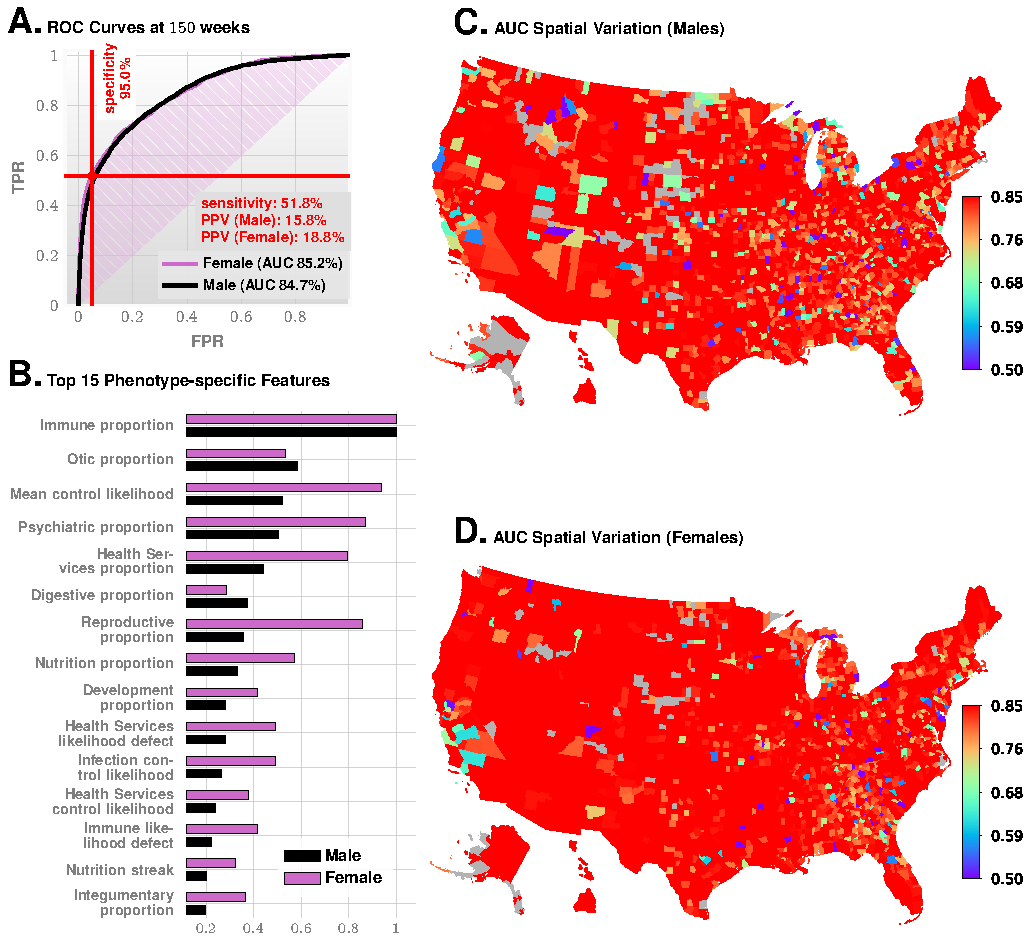
\includegraphics[width=0.85\textwidth]{Figures/External/perfA.pdf}
  \fi

  \captionN{Predictive Performance. Panel %C shows the distribution of the AUC, and panel
    A shows the ROC curves for males and females. Panel B shows the feature importance inferred by our prediction pipeline. The detailed description of the features is given in Table~\ref{EXT-tab1}. The most import feature is related to immunologic disorders, and we note that in addition to features related to individual disease categories, we also have the mean control likelihood (rank 3), which may be interpreted as the average likelihood of the diagnostic patterns correspond to the control category as opposed to the \treatment category. Panels C and D show the spatial variation in the achieved predictive performance at 150 weeks, measured by AUC, for males and females, respectively. Gray areas lack data on either positive or negative cases. These county-specific AUC plots show that the performance of the algorithm has  relatively weak geospatial dependence, which is important in the light of current uneven distribution of diagnostic resources.
  }\label{fig1}
\end{figure*}
\else
\refstepcounter{figure}\label{fig1}
\fi
% ###########################################################
% ###########################################################
% ###########################################################
% ###########################################################
\ifFIGS
\begin{figure*}[!ht]
  \tikzexternalenable
  \tikzsetnextfilename{perfB}
  
  \centering 
  \def\DATA{../../data_revision}
  \iftikzX
  \input{Figures/figpred2_}
  \else
  \includegraphics[width=0.85\textwidth]{Figures/External/perfB.pdf}
  \fi

  \captionN{\textbf{More details on Predictive Performance and Variation of Inferred Risk.} Panel A illustrates AUC achieved as a function of
    patient age, for the Truven and UCM datasets. The shaded area outlines the 2 - 2.5  years of age, and  shows that we achieve $>80\%$ AUC for either sex from shortly after 2 years.   Panel B illustrates how the average risk changes with time for the control and the positive cohorts. Panel C shows the distribution of the prediction horizon: the time to a clinical diagnosis after inferred  relative risk crosses $90\%$. Panel D shows that for each new disease code for a low-risk child, ASD risk increases by approximately $2\%$ for either sex. Panel E illustrates the risk progression of a specific, ultimately autistic male child in the Truven database. Abbreviations in the legend: ill defn. (Symptoms, Signs, And Ill-Defined Conditions),   musc. skltl. (Diseases Of The Musculoskeletal System And Connective Tissue), cond. orig. in perintl. (Certain Conditions Originating In The Perinatal Period), immun. (Endocrine, Nutritional And Metabolic Diseases, And Immunity Disorders), nerv. \& sensory (Diseases Of The Nervous System And Sense Organs), respir. (Respiratory Disorders), and digest. (Digestive Disorders). Panel F illustrates  how inferred models differ between the control vs. the \treatment cohorts. On average, models get less complex, implying the exposures get more statistically independent.}\label{fig2}
\end{figure*}
\else
\refstepcounter{figure}\label{fig2}
\fi
% ###########################################################
% ###########################################################
% ###########################################################
\ifFIGS
% ###########################################################
\begin{figure}[!ht]
  \tikzexternalenable
  \tikzsetnextfilename{perfCv}

  \centering
  
  \def\AXISCOL{white}
  \def\TEXTCOL{gray}
  \iftikzX
  \input{Figures/figprcv_.tex}
  \else
  \includegraphics[width=0.75\textwidth]{Figures/External/perfCv.pdf}
  \fi

  \captionN{\textbf{Metrics relevant to clinical practice: PPV vs Sensitivity trade-offs.} Panel A shows the precision/recall curves, $i.e.$,  the trade-off between PPV and sensitivity. Panel B shows how we can boost performance using population stratification from the distribution of M-CHAT/F scores in the population, as reported by the CHOP study~\cite{pmid31562252}. Panel C illustrates the boosted performance compared to M-CHAT/F alone,
    measured by the relative percentage increase in sensitivity, and percentage decrease in positive screens. Note that the population prevalence impacts this optimization, and hence  we have  a distinct  curve for each prevalence value ($1.7\%$ is the CDC estimate, while $2.23\%$ is reported by the CHOP study).  The two extreme operating zones marked as High Precision (HP) and High Recall (HR): if we choose to operate in HR, then we do not reduce the number of positive screens by much, but maximize sensitivity, while by operating in HP, we do not increase sensitivity by much but double the PPV achieved in current practice. Note in all these zones, we maintain specificity above $95\%$, which is the current state of art, implying that by doubling the PPV, we can halve the number of positive screens currently reported, thus potentially sharply reducing the queues and wait-times. }\label{figprc}
\end{figure}

% ###########################################################
\else
\refstepcounter{figure}\label{figprc}
\fi 
% ###########################################################
% ##########################################
% ####################################
\def\RCOL{\rowcolor{teal!40}}
%#################################### 
\begin{table*}[!ht]
  \captionN{Standalone and Combined Performance}
\begin{subtable}{\textwidth}
\centering 
\captionN{Standalone PPV Achieved at 100, 112 and 150 Weeks For Each Dataset and Gender {\bf (M-CHAT/F:  sensitivity=$38.8\%$, specificity=$95\%$, PPV=$14.6\%$ between 16 and  26 months ($\approx$112 weeks))}}\label{EXT-tabssp}

  \vskip .5em

\begin{tabular}{L{.75in}|L{.75in}|L{.75in}|L{.5in}|L{.5in}|L{.75in}}
\hline
week&spec.&sens.&PPV&sex&dataset\\\hline
100&0.92&0.39&0.14&F&UCM\\\hline
100&0.95&0.39&0.19&M&UCM\\\hline
100&0.93&0.39&0.13&F&Truven\\\hline
100&0.91&0.39&0.10&M&Truven\\\hline
%\RCOL 112&0.94&0.35&0.17&F&UCM\\\hline
\RCOL 112&0.93&0.39&0.16&F&UCM\\\hline
\RCOL 112&0.95&0.39&0.20&M&UCM\\\hline
\RCOL 112&0.96&0.39&0.22&F&Truven\\\hline
\RCOL 112&0.95&0.39&0.17&M&Truven\\\hline
% 150&0.94&0.39&0.19&F&UCM\\\hline
% 150&0.98&0.39&0.34&F&Truven\\\hline
% 150&0.97&0.39&0.26&M&Truven\\\hline
% 150&0.97&0.39&0.26&M&UCM\\\hline

\end{tabular}\end{subtable}
\vskip 1em
\begin{subtable}{\textwidth}
\centering
\captionN{Personalized Operation Conditioned on M-CHAT/F Scores at  26 months}\label{EXT-tabboost}
  \vskip .5em

\begin{tabular} {L{.33in}|L{.33in}|L{.33in}|L{.33in}||L{.35in}|L{.35in}|L{.375in}||L{.375in}|L{.35in}|L{.35in}||L{.6in}}
\hline
\multicolumn{4}{c||}{\cellcolor{lightgray!60}M-CHAT/F Outcome}  & \multicolumn{3}{c||}{\mnp{.9in}{\vskip .2em global performance (Truven)\vskip .2em  } }&\multicolumn{3}{c||}{\mnp{1in}{\vskip .2em global performance\\(UCM)\vskip .2em }} &  \multirow{3}{*}{prevalence$^\star$}\\\cline{0-9}
 0-2  NEG & 3-7  NEG & 3-7  POS & $\geq  8$  POS & \multirow{2}{*}{\mnp{.1in}{speci-ficity}} & \multirow{2}{*}{\mnp{.1in}{sensi-tivity}} &\multirow{2}{*}{PPV}& \multirow{2}{*}{\mnp{.1in}{speci-ficity}} & \multirow{2}{*}{\mnp{.1in}{sensi-tivity}} & \multirow{2}{*}{PPV} & \\\cline{0-3}
\multicolumn{4}{c}{\cellcolor{lightgray} specificity choices}  & & & &&&&\\\hline 
  0.2&0.54&0.83&0.98&0.95&0.585&0.209&0.95&0.505&0.186&0.022\\\hline 
0.21&0.53&0.83&0.98&0.95&0.586&0.208&0.95&0.506&0.184&0.022\\\hline 
0.42&0.87&0.98&0.99&\cellcolor{\PCOL}0.98&\cellcolor{\PCOL}0.433\cellcolor{\PCOL}&\cellcolor{\PCOL}0.331&0.98&0.347&0.284&0.022\\\hline 
0.48&0.87&0.97&0.99&\cellcolor{\PCOL}0.98&\cellcolor{\PCOL}0.432&\cellcolor{\PCOL}0.331&0.98&0.355&0.289&0.022\\\hline 
0.38&0.54&0.94&0.98&\cellcolor{\PCOL}0.95&\cellcolor{\PCOL}0.736\cellcolor{\PCOL}&\cellcolor{\PCOL}0.203&0.95&0.628&0.178&0.017\\\hline 
0.3&0.55&0.94&0.98&\cellcolor{\PCOL}0.95&\cellcolor{\PCOL}0.737&\cellcolor{\PCOL}0.203&0.95&0.633&0.179&0.017\\\hline 
0.58&0.96&0.98&0.99&0.98&0.492&0.302&0.98&0.373&0.247&0.017\\\hline 
0.59&0.96&0.98&0.99&0.98&0.491&0.303&0.98&0.372&0.248&0.017\\\hline 
0.46&0.92&0.97&0.99&0.977&0.534&0.291&0.977&0.448&0.256&0.017\\\hline 
0.48&0.92&0.97&0.99&0.978&0.533&0.292&0.978&0.448&0.257&0.017\\\hline 
 
\end{tabular}
\vskip 1em

\flushleft
$^\star$Prevalence reported by CDC is $1.7\%$, while the CHOP study reports a value of $2.23\%$. The results of our optimization depend on the prevalence estimate.
\end{subtable}
\end{table*}  
%####################################
%###########################################################
%###########################################################
\ifFIGS
\begin{figure*}[!t]
  \tikzexternalenable
    \tikzsetnextfilename{comorbidA}

\def\DATA{../../data_latest}
\iftikzX
 \input{Figures/figClass0_.tex}
 \else
  \includegraphics[width=0.9\textwidth]{Figures/External/comorbidA}
\fi
  \vspace{-5pt}
  
  \captionN{\textbf{Co-morbidity Patterns} Panel A and B. Difference in occurrence frequencies of diagnostic codes between true positive (TP) and true negative (TN) predictions. The dotted line on panel B shows the  abscissa lower cut-off in Panel A, illustrating the lower prevalence of codes in females. Panel C illustrates log-odds ratios for ICD9 disease categories at different ages. Importantly, the negative associations disappear when we consider older children, consistent with the lack of such reports in the literature which lack studies on very young cohorts. }\label{EXT-fig3}
  \vspace{-5pt}
  
\end{figure*}
\else
\refstepcounter{figure}\label{EXT-fig3}
\fi
% ###########################################################
% #############
